\documentclass[../main.tex]{subfiles}
\begin{document}
Quando parliamo di livelli logici non si considerano i valori continui ma soltanto quelli discreti.
Immaginiamo un grafico in cui per ogni valore di $x$ la $y$ può essere soltanto 1 o 0.

Se però abbiamo un valore intermedio (nè 1 nè 0), la lettura del valore diventerebbe ambigua
\begin{figure}[h]
    \centering
    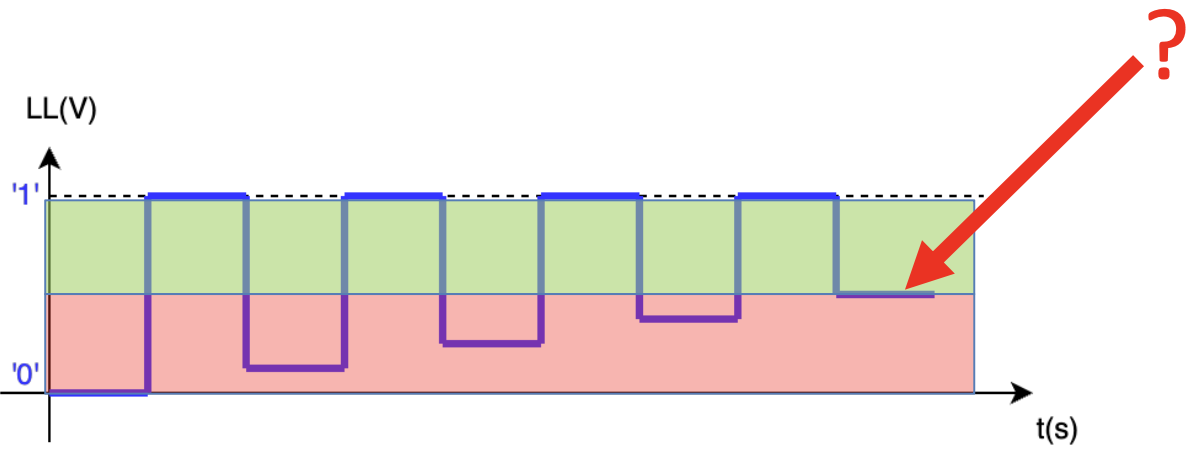
\includegraphics[width=0.5\textwidth]{images/logicLevels.png}
    \caption{Livelli logici reali}
\end{figure}

\subsection{Rumore}
Questi valori intermedi possono esseri causati dal rumore. Il rumore è tutto ciò che disturba il segnare
è può alterare il valore logico durante il passaggio di input o do output.
\begin{figure}[h]
    \centering
    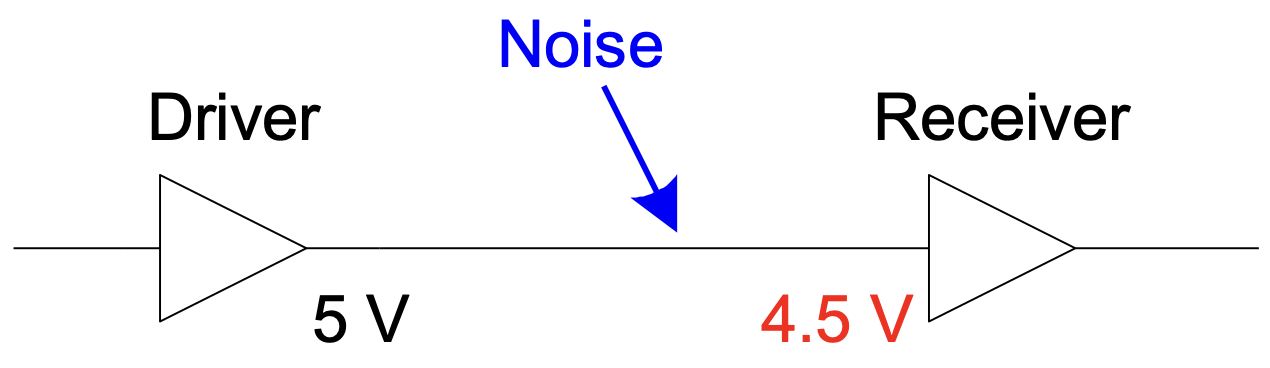
\includegraphics[width=0.5\textwidth]{images/rumore.png}
    \caption{Esempio di rumore}
\end{figure}

\subsection{Margini del rumore}
Prendendo come riferimento l'immagine sopra, definiamo i concetti di \textbf{Voltage output high/low ($V_{OH}, V_{OL}$)} e \textbf{Voltage input high/low ($V_{IH, V_{IL}}$)}.
Essi definiscono i range di valori per l'1 logico e lo 0 logico rispettivamente in entrata e in uscita.

Le differenza tra tensione di uscita del driver e tensione d'entrata del receiver viene chiamata \textbf{Noise Margin ($NM_H$ e $NM_L$)}.

\begin{figure}[h]
    \centering
    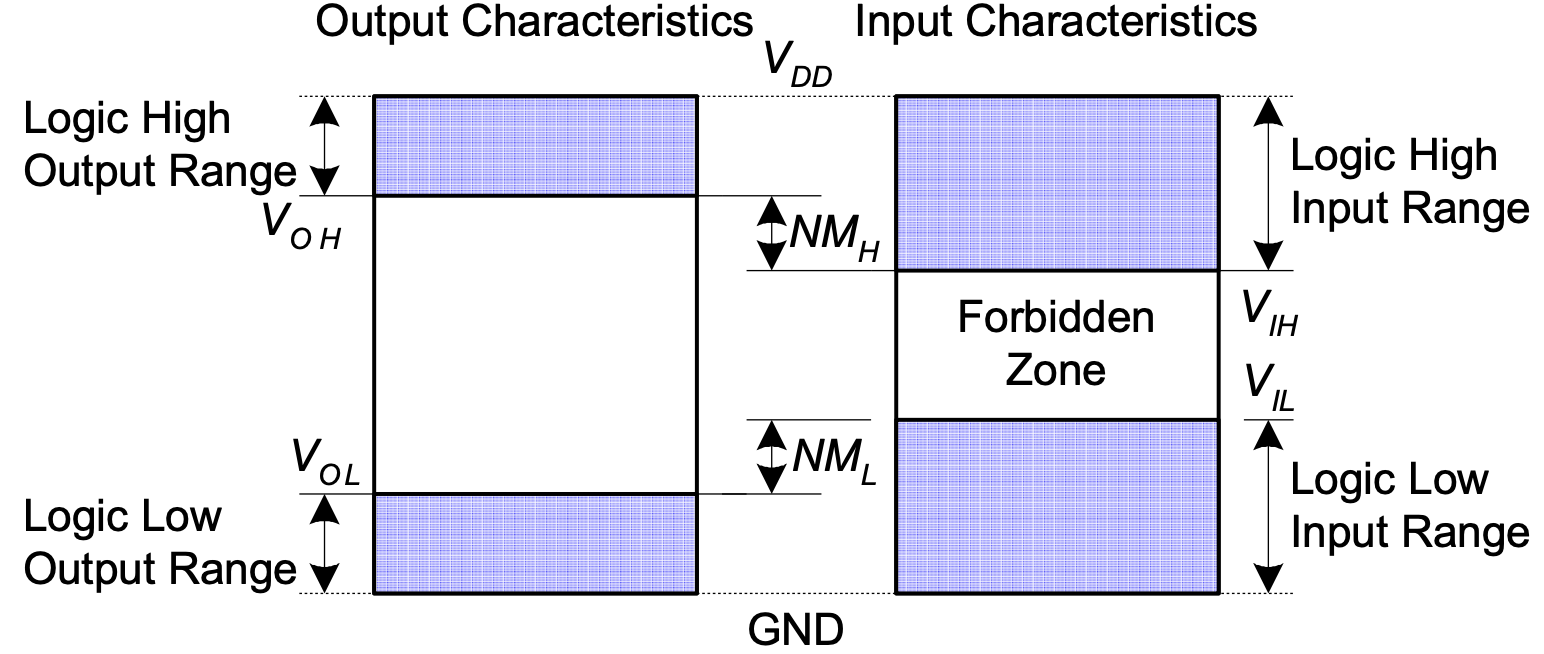
\includegraphics[width=0.6\textwidth]{images/noiseMargin.png}
    \caption{Schema noise margins}
\end{figure}
Se un valore logico non rientra nei margini esso entra nella \textbf{forbidden zone}, è importante definire bene questa zona. 
Se essa è troppo piccola si avrà uno scenario simile a quello iniziale, in cui non si sa che valore logico assegnare, se invece
è troppo grande in caso di rumore si ha il rischio di non poter leggere il valore.

Per calcolare questi margini in generale valore
\begin{align*}
    NM_H &= V_{OH} - V_{IH} \\
    NM_L &= V_{IL} - V_{OL}
\end{align*}

\end{document}